\documentclass{article}
\usepackage{amsmath}
\usepackage{xspace}
\usepackage{tikz}
\usetikzlibrary{positioning, arrows.meta, bending}
\newcommand{\NT}{\ensuremath{N_{\rm T}}\xspace}
\newcommand{\NTt}{\ensuremath{N_{\rm T}^{\rm t}}\xspace}
\newcommand{\NTtt}{\ensuremath{N_{\rm T}^{\rm t'}}\xspace}
\newcommand{\NTm}{\ensuremath{N_{\rm T}^{\rm m}}\xspace}
\newcommand{\nevhat}{\ensuremath{\hat{n}_{\rm ev}}\xspace}
\newcommand{\nev}{\ensuremath{n_{\rm ev}}\xspace}
\begin{document}
	\begin{figure}[h]
		\centering
		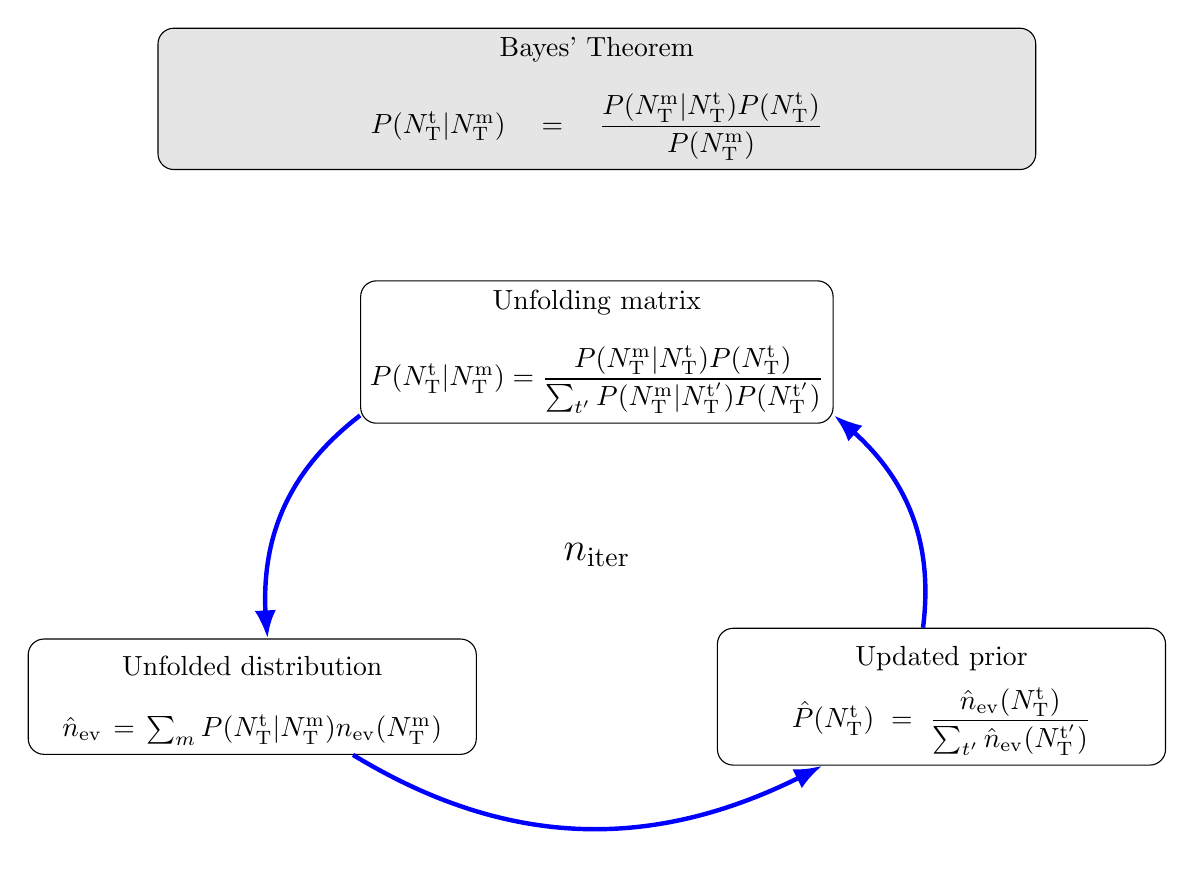
\begin{tikzpicture}[node distance=1.4cm,box/.style={draw, rounded corners=.2cm}]
			%\node[box, text width=0.9\textwidth, align=center] (eqn) {\NTt ...\ true multiplicity};
			%below=of eqn
			\node[box, fill=black!10, text width=0.9\textwidth, align=center] (thm) {Bayes' Theorem\\\vspace{1em}$P(\NTt | \NTm) = \dfrac{P(\NTm | \NTt)P(\NTt)}{P(\NTm)}$};
			\node[box, below=of thm, align=center] (f1) {Unfolding matrix\\
			\\$P(\NTt | \NTm) = \dfrac{P(\NTm | \NTt)P(\NTt)}{\sum_{t'}P(\NTm | \NTtt)P(\NTtt)}$};
			\node[draw=none, below=of f1, align=center] (f2) {\begin{Large}$n_\mathrm{iter}$\end{Large}};
			\node[draw=none, below=of f2, align=center] (f0) {};
			\node[box, left=of f0, text width=.45\textwidth,text height=1em, align=center] (f3) {Unfolded distribution\\\vspace{1em}$\nevhat = \sum_m P(\NTt | \NTm) \nev(\NTm)$};
			\node[box, right=of f0, text width=.45\textwidth, text height=1em, align=center] (f4) {Updated prior\\\vspace{0.5em}$\hat{P}(\NTt) = \dfrac{\nevhat(\NTt)}{\sum_{t'} \nevhat(\NTtt)}$};
			\draw[-{Latex[bend]}, ultra thick, blue] (f1) to[bend right] (f3);
			\draw[-{Latex[bend]},ultra thick, blue] (f3) to[bend right] (f4);
			\draw[-{Latex[bend]},ultra thick, blue] (f4) to[bend right] (f1);
		\end{tikzpicture}
		\caption{Diagram showing the algorithm for calculating something}
	\end{figure}
\end{document}